\chapter{Brugervejledning og eksempel}

\section{Forestillinger}

\subsection{Åben Bookie}

Når "Bookie" bliver kørt, kommer man direkte ind på programmets brugergrænseflade. Dog er det ikke muligt at se salene, da der indtil videre ikke er blevet valgt nogen forestilling. Forestillingerne har et forhold til salene, men ikke omvendt. \ref{screenshot: bookie} viser Bookie's startside, hvor der også er muligt at se feltet, hvor ekspedienten kan indtaste kundens telefonnummer og derefter reservere billetter. Dette kan dog først gennemføres efter at en forestilling er valgt. 

\begin{figure}[h]
  \centering
  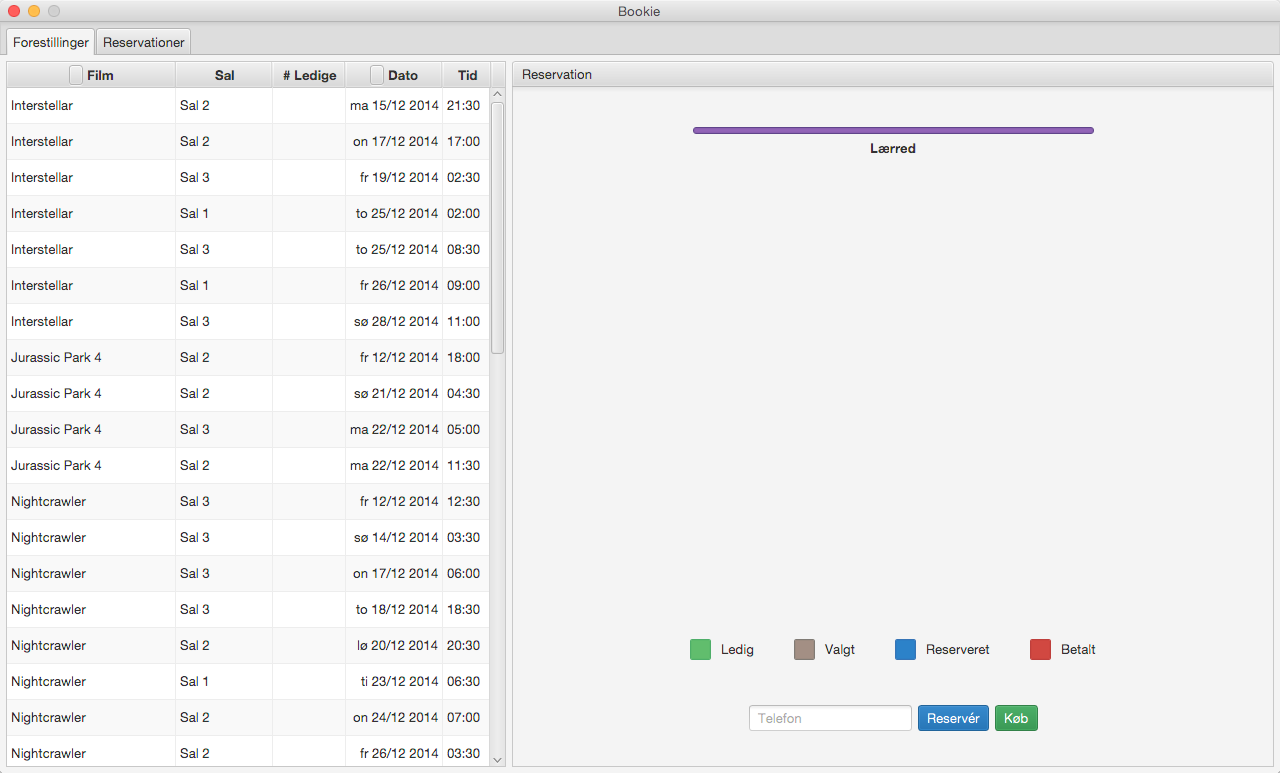
\includegraphics[width=\textwidth]{bookie.png}
  \caption{Bookie startside}
  \label{screenshot: bookie}
\end{figure}

\subsection{Vælg forestilling}

Der er muligt at sortere efter hvilken film kunden vil se, hvilken sal han/hun vil se den i eller hvilken dag/tidspunkt. Uanset hvilken ønske kunden har, så kan ekspedienten hurtigt og nemt trykke på baren med den ønskede kolonne, hvorefter det valgte element bliver sorteret.

I dette eksempel er der blevet sorteret efter film, hvorefter der er blevet valgt en forestilling (\ref{screenshot: chosen-showtime}), og det er nu muligt at se den tilhørende sal med tilhørende sæder.

\begin{figure} [h]
  \centering
  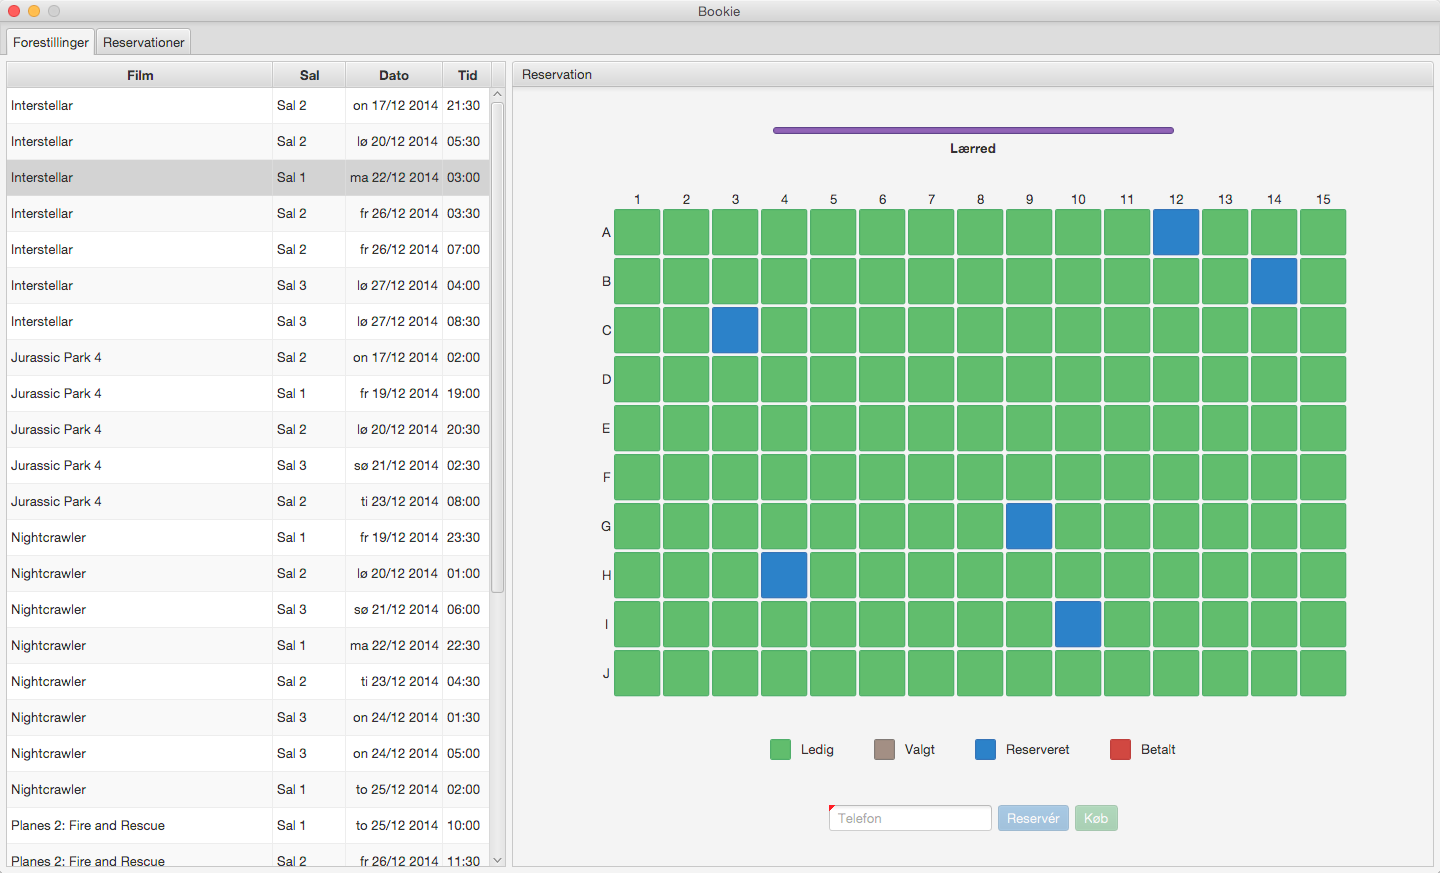
\includegraphics[width=\textwidth]{chosen-showtime.png}
  \caption{Den valgte forestilling: Interstellar}
  \label{screenshot: chosen-showtime}
\end{figure}

\newpage

\subsection{Vælg sæder}

Sæderne er angivet i rækker og kolonner, hvor rækkerne har fået navne efter alfabetet og kolonnerne efter tal. Dette gør det meget nemt at beskrive hvor i salen de valgte sæder befinder sig. Holder ekspedienten musen hen over et af de grønne sæder, og trykker på det, resulterer det i at sædet får en grå farve (dette kan også ses i legenden i \ref{screenshot: chosen-seats}).

\begin{figure} [h]
  \centering
  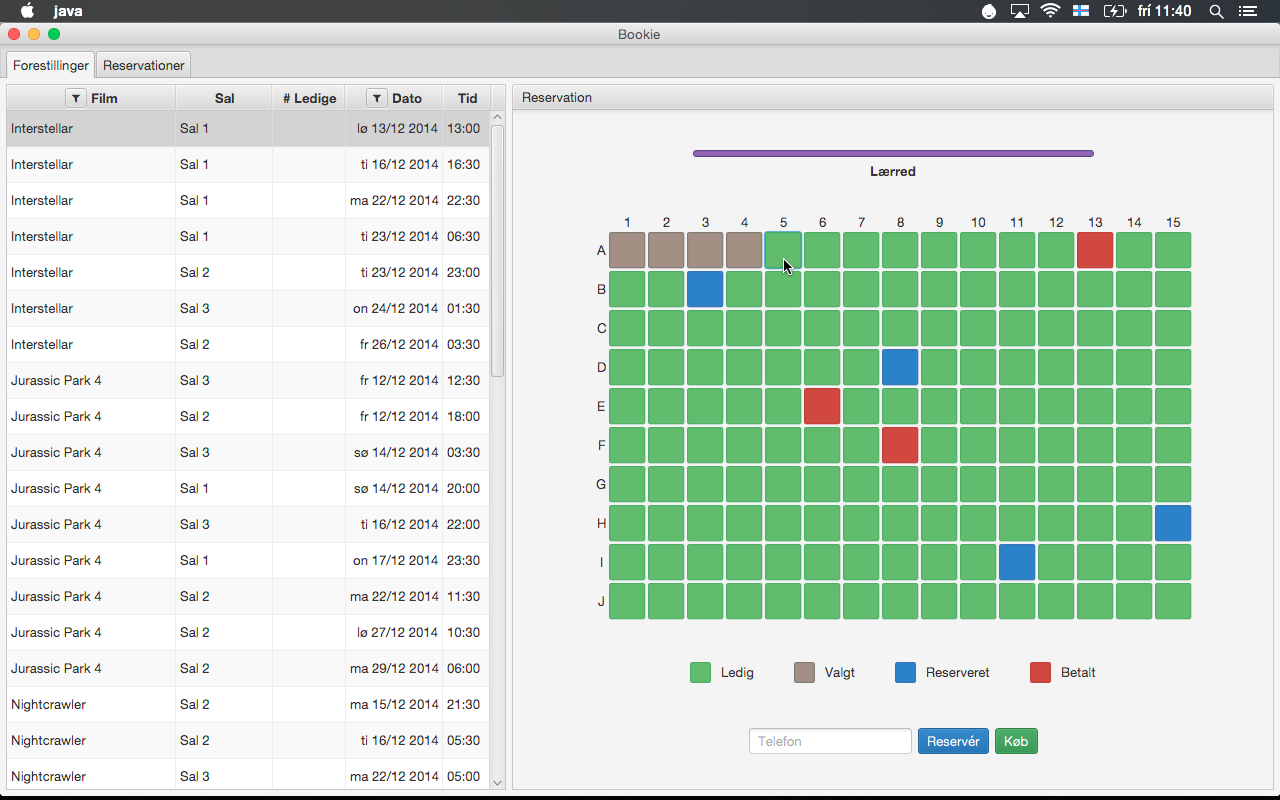
\includegraphics[width=0.4\textwidth]{chosen-seats.png}
  \caption{Valgte sæder}
  \label{screenshot: chosen-seats}
\end{figure}

\subsection{Indtast telefonnummer}

Efter at sæderne er blevet valgte, er det muligt at indtaste et telefonnummer (\ref{screenshot: phone-number}). Trykker man derefter på \textit{Reservér} knappen, ændrer sæderne farve og bliver blå. Hvilket viser ekspedienten, at reservationen er gennemført. Ses også i \ref{screenshot: booked-seats}

\begin{figure} [h]
  \centering
  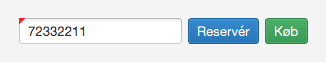
\includegraphics[width=0.4\textwidth]{phone-number.png}
  \caption{Telefonnummer bliver indtastet.}
  \label{screenshot: phone-number}
\end{figure}

\begin{figure} [h]
  \centering
  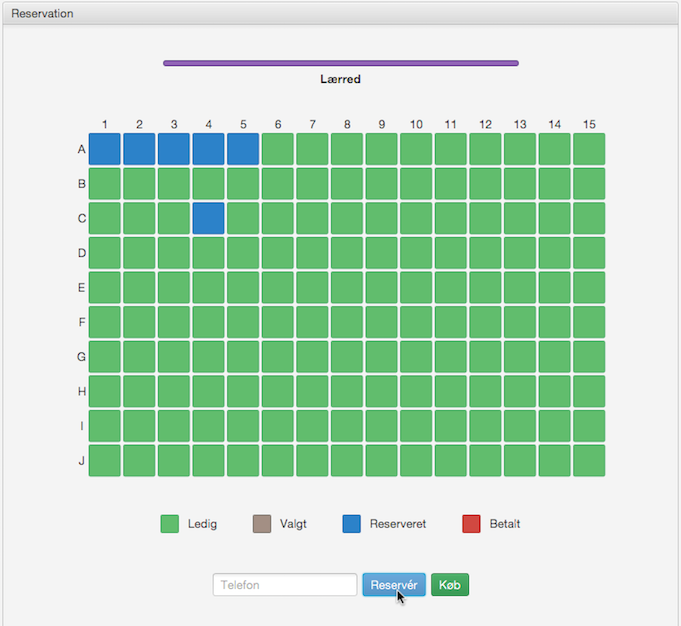
\includegraphics[width=0.4\textwidth]{booked-seats.png}
  \caption{Reserverede sæder.}
  \label{screenshot: booked-seats}
\end{figure}

\section{Reservationer}

\subsection{Gå til Reservationer}
Efter at sæderne er reserverede, er der blevet oprettet billetter inde i Reservationer. Alle de eksisterende reservationer kan ses inde på \textit{Reservationer} oppe i venstre hjørne (\ref{screenshot: go-to-reservations}).

\begin{figure} [h]
  \centering
  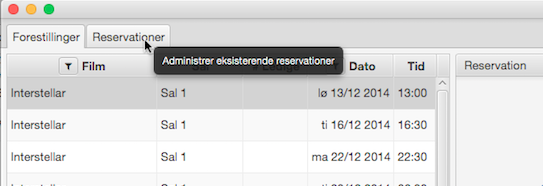
\includegraphics[width=0.4\textwidth]{go-to-reservations.png}
  \caption{Gå til alle reservationer.}
  \label{screenshot: go-to-reservations}
\end{figure}

Alle reservationerne er vist på en liste, som er mulig at sortere efter eget valg. Både film, dag/tidspunkt, sal, antal billetter (hvis ekspedienten evt. skulle få lyst til det). 

\begin{figure} [h]
  \centering
  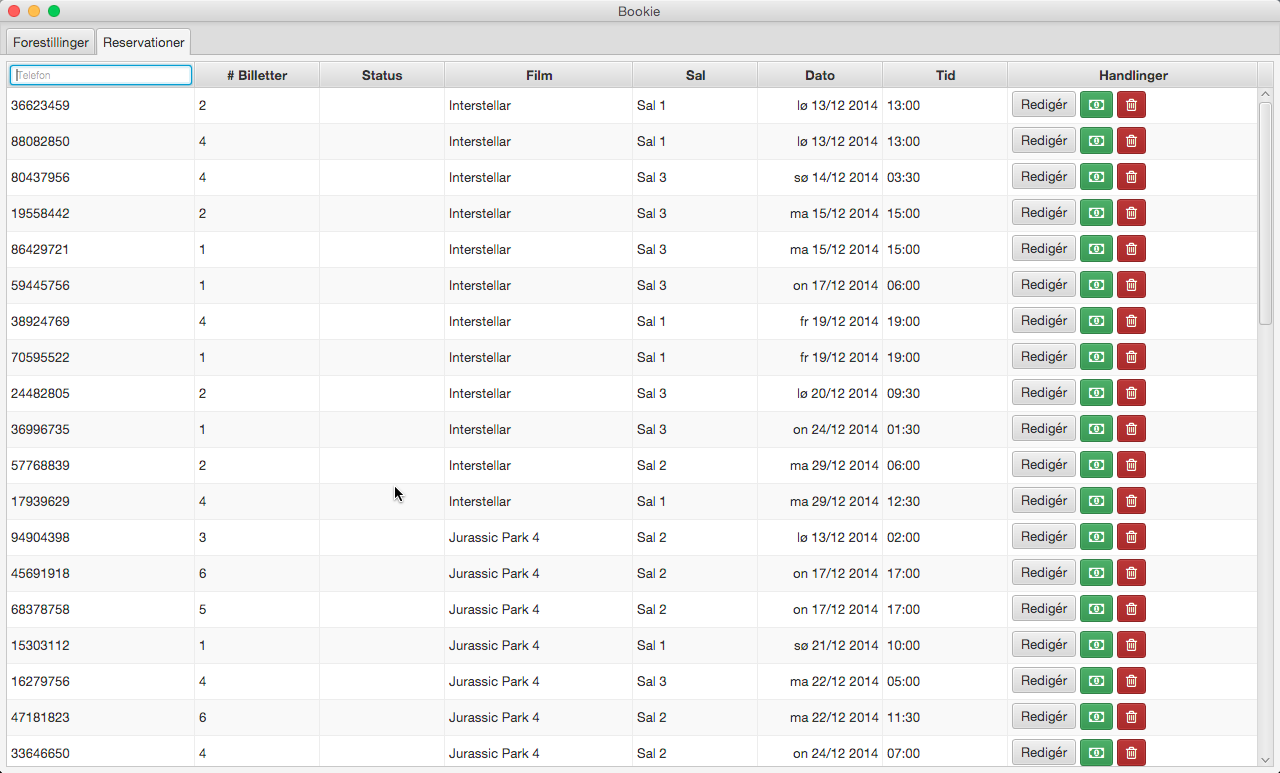
\includegraphics[width=0.4\textwidth]{all-reservations.png}
  \caption{Alle reservationer bliver vist.}
  \label{screenshot: all-reservations}
\end{figure}

\subsection{Filtrering af telefonnumre}

Øverst i venstre hjørne af denne side er der et felt til filtrering af telefonnumrene (\ref{screenshot: filter3}). Dette gør det overskueligt at finde den enkelte reservation, når den skal redigeres eller slettes. 

\begin{figure} [h]
  \centering
  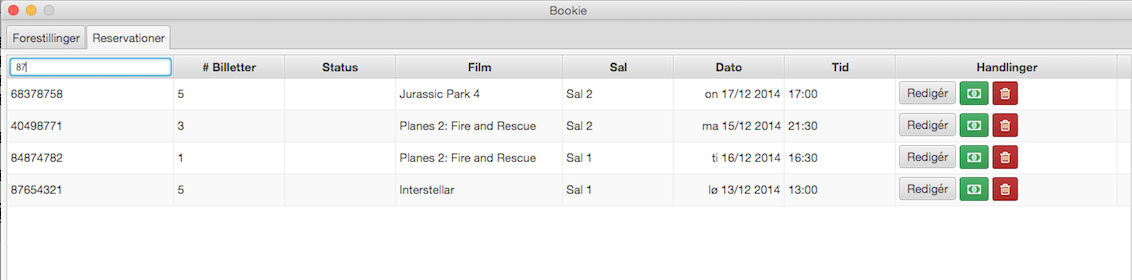
\includegraphics[width=0.4\textwidth]{filter3.png}
  \caption{Filtrering af telefonnumre.}
  \label{screenshot: filter3}
\end{figure}

\subsection{Redigering af reservationer}

Når den eftersøgte reservation er fundet via filtreringen, kan ekspedienten hurtigt redigere dem ved at trykke på knappen ude i højre side (\ref{screenshot: edit-button}. Ekspedienten kommer nu igen ind på \textit{Forestillinger}-siden og kan tilføje reservationer til de enkle forestillinger (\ref{screenshot: edit1}).

\begin{figure} [h]
  \centering
  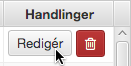
\includegraphics[width=0.4\textwidth]{edit-button.png}
  \caption{Mulighed for at redigere den enkelte reservation.}
  \label{screenshot: edit-button}
\end{figure}

\begin{figure} [h]
  \centering
  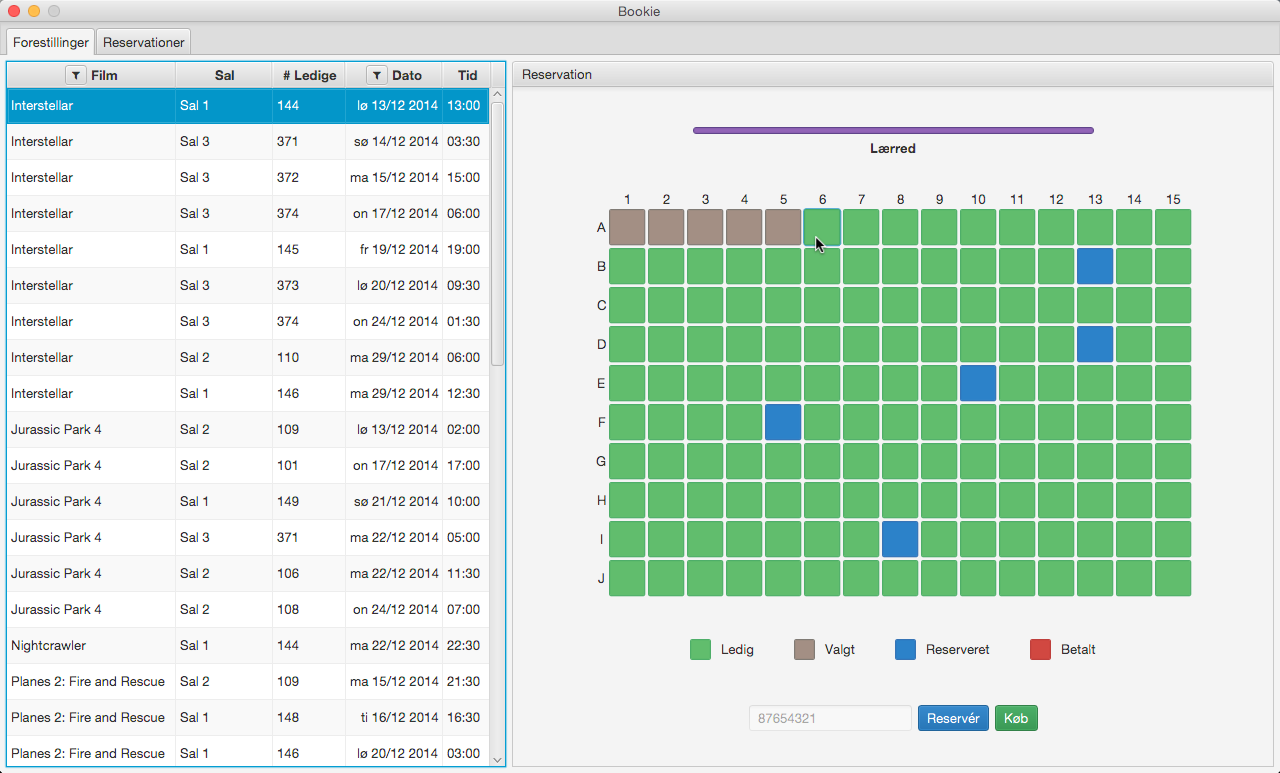
\includegraphics[width=0.4\textwidth]{edit1.png}
  \caption{Efter der er blevet trykket på \textit{Redigér}-knappen}
  \label{screenshot: edit1}
\end{figure}


Hvis det skulle ske, at kunden vil ændre reservationen således, at han/hun vil se den valgte film på et andet tidspunkt, så vil ekspedienten slette hele reservationen og oprette en ny, da Bookie ikke er lavet til at flytte reservationerne fra tidspunkt til tidspunkt.

\subsection{Sletning af reservationer}

At slette er reservation er lige så smertefrit som at arbejde resten af Bookie. Bliver der trykket på den røde knap med skraldespand-ikonet ved siden af \textit{redigér} knappen (som ses på \ref{screenshot: delete-button}, så kommer et pop-up (\ref{screenshot: delete-reservation}, hvor man kan vælge mellem \textit{cancel} eller \textit{ok}. Vælger ekspedienten \textit{cancel}, sker der ikke noget andet end, at pop-up'et forsvinder og \textit{Reservationer} forbliver som før. Vælger ekspedienten \textit{ok}, forsvinder den valgte reservation fra listen (\ref{screenshot: after-delete}).

\begin{figure} [h]
  \centering
  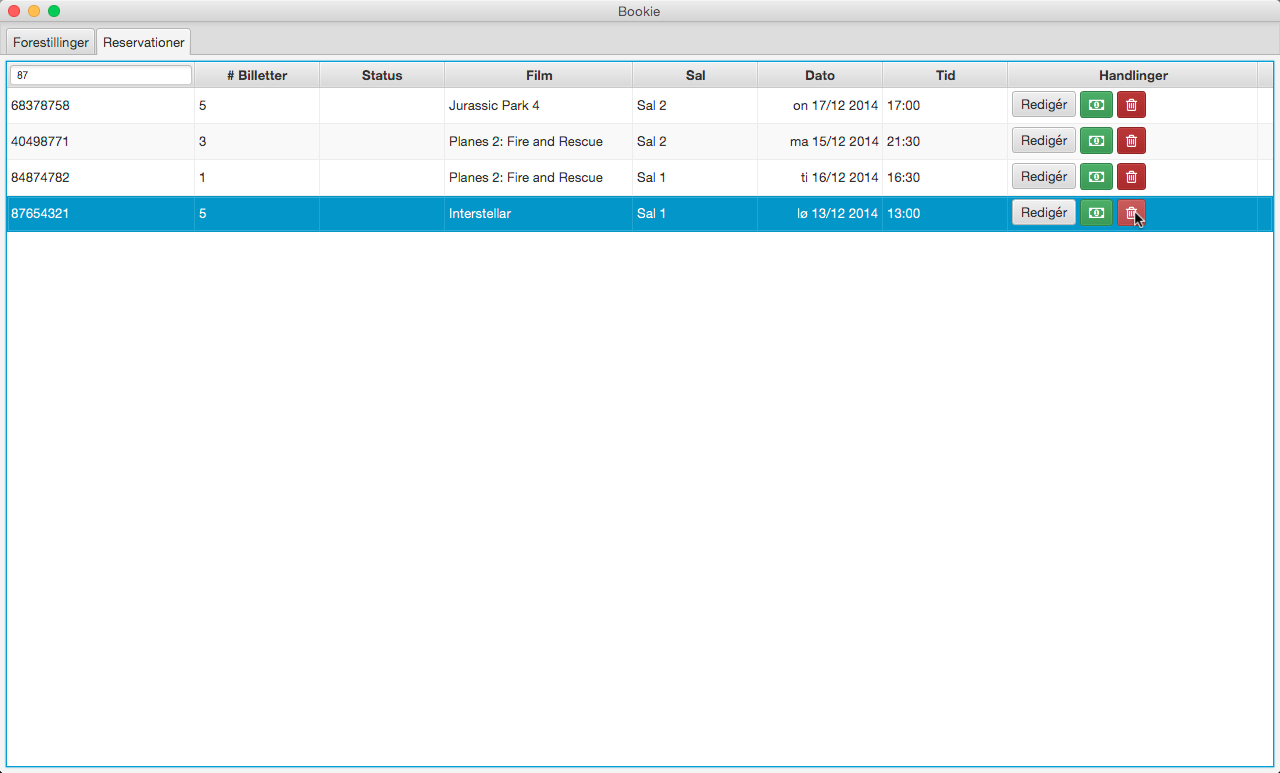
\includegraphics[width=0.4\textwidth]{delete-button.png}
  \caption{Mulighed for at slette den enkelte reservation.}
  \label{screenshot: delete-button}
\end{figure}

\begin{figure} [h]
  \centering
  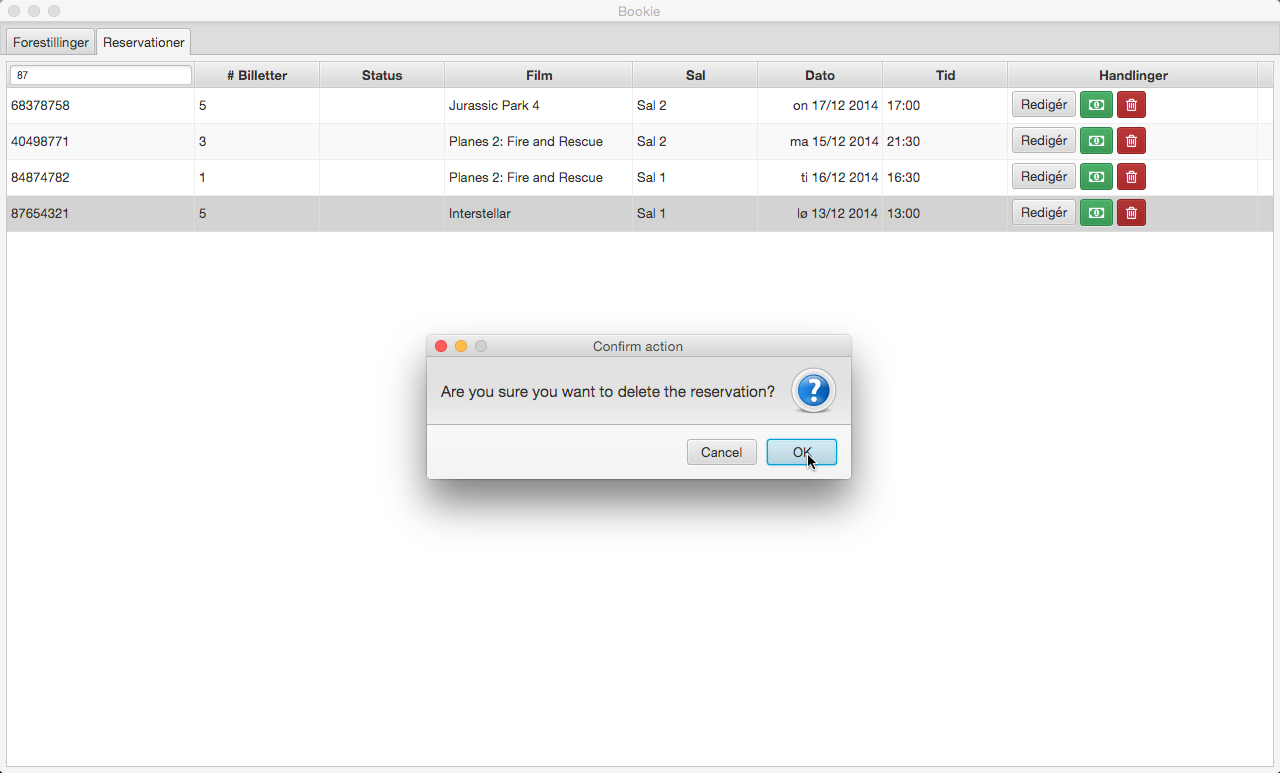
\includegraphics[width=0.4\textwidth]{delete-reservation.png}
  \caption{Sletning af reservation.}
  \label{screenshot: delete-reservation}
\end{figure}

\begin{figure} [h]
  \centering
  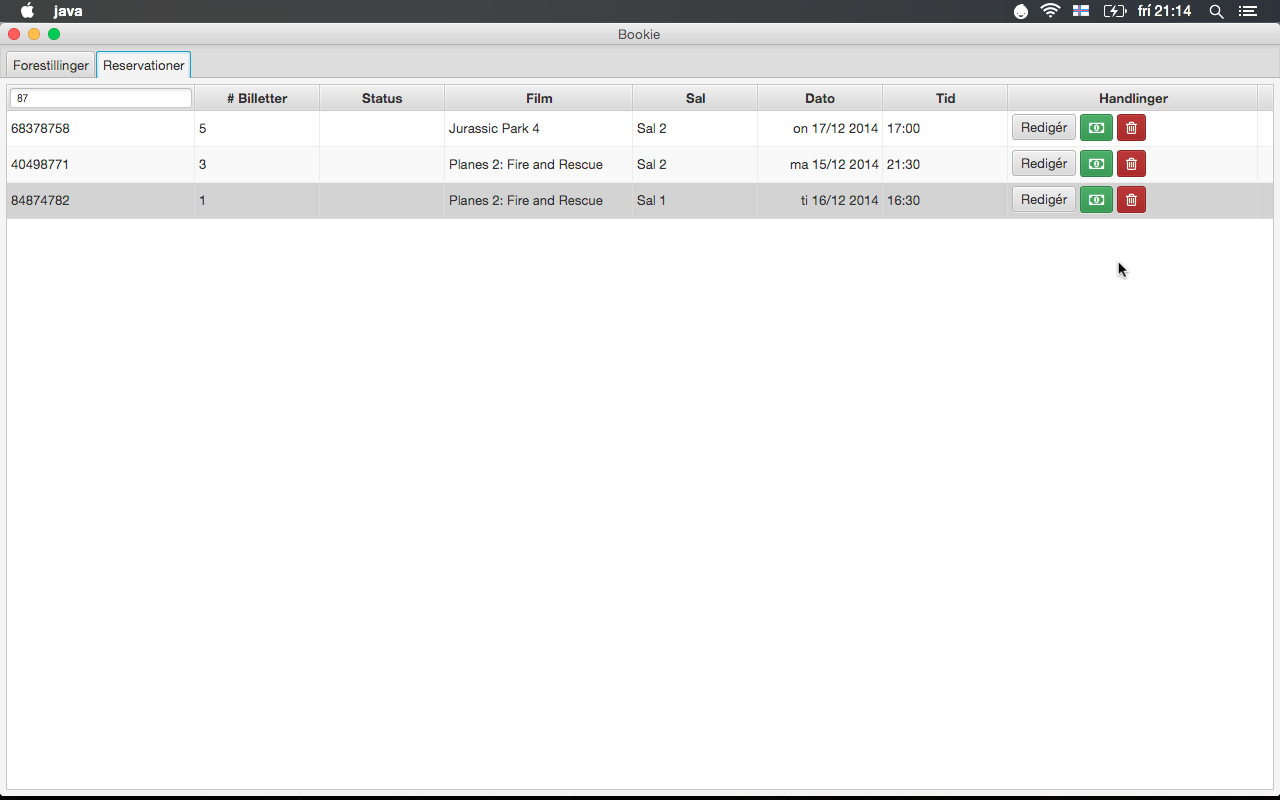
\includegraphics[width=0.4\textwidth]{after-delete.png}
  \caption{Efter at en reservation er slettet.}
  \label{screenshot: after-delete}
\end{figure}

Det viser sig, at det er meget nemt for ekspedienten at finde rundt i Bookie. Hvilket er meget godt, da der kan være meget pres, f.eks. til premieren til \textit{The Hobbit - The Battle of the Five Armies} her i december måned. Selv om der kun er én ekspedient der kan bruge Bookie ad gangen, så må man kunne holde hovedet koldt, når der skal serviceres en billetluge og en telefon på samme tid.